% =====================================================================
% Nanograph: A Structural Graph Representation for Curvilinear Microscopy
% MICCAI-style (Springer LNCS). Compiles on Overleaf with the LNCS class
% (no local TeX on the compute node). Select "LNCS" template or add
% llncs.cls + splncs04.bst to the project.
% =====================================================================
\documentclass[runningheads]{llncs}

\usepackage{graphicx}
\usepackage{booktabs}
\usepackage{amsmath}
\usepackage{amssymb}
\usepackage{xcolor}
\usepackage[hidelinks]{hyperref}
\usepackage{xspace}

\newcommand{\method}{\textsc{Nanograph}\xspace}

\title{Nanograph: A Structural Graph Representation of\\ Curvilinear Microscopy Images}
\titlerunning{Nanograph: Structural Graphs for Curvilinear Microscopy}

\author{Anonymous}
\authorrunning{Anonymous}
\institute{Anonymous Institution}

\begin{document}
\maketitle

% ---------------------------------------------------------------------
\begin{abstract}
Modern microscopy routinely images \emph{curvilinear} structures---mitochondrial
networks, blood vessels, microtubules and neurites---as dense pixel arrays that
are storage-heavy and, crucially, not structure-aware: downstream morphometric
and topological analysis must re-extract the geometry every time. We present
\method, a pipeline that converts a curvilinear microscopy image into an explicit
\emph{attributed graph}. Nodes carry position, width, intensity and local
orientation; edges carry connectivity, length, curvature and mean width. The
resulting object is simultaneously (i) \emph{compact} (a few kilobytes per
image), (ii) directly \emph{analysable} (morphometry and $\beta_0/\beta_1$
topology are read off the graph), and (iii) \emph{reconstructable} through
orientation-aligned point-spread functions. On 726 fluorescence organelle
images \method encodes each image in $\approx$\,2.5\,kB and reconstructs the
foreground at 28.4\,dB FG-PSNR / 0.997 FG-SSIM, beating byte-matched JPEG on
reconstruction IoU for 77\% of images. The representation transfers across five
microscopy modalities. We further analyse the pipeline's dominant bottleneck,
foreground segmentation: a centreline-aware (clDice) U-Net lifts held-out
segmentation IoU from 0.38 to 0.88 in-domain, and a \emph{polarity-agnostic}
multi-domain retraining restores segmentation on four out-of-domain curvilinear
datasets---including electron-microscopy mitochondria, where classical
thresholding scores 0.001 IoU and the retrained network reaches 0.82.
\keywords{Structural representation \and Curvilinear structures \and Image
compression \and Graph \and Segmentation \and Microscopy.}
\end{abstract}

% =====================================================================
\section{Introduction}
% =====================================================================
High-throughput microscopy produces vast collections of images whose biological
content is \emph{curvilinear}: mitochondrial networks, cytoskeletal filaments,
retinal vasculature and neuronal arbours are all thin, branching, one-dimensional
structures embedded in a two-dimensional field. Two problems follow from storing
such data as raster images. First, generic image codecs (JPEG, PNG) are tuned for
natural-image statistics and spend most of their bit budget on texture and
background that are biologically irrelevant. Second---and more importantly for
analysis---a pixel array is not \emph{structure-aware}: every downstream task
(branch counting, length and width statistics, connectivity, tracking across
time) must first re-derive the geometry, and does so from scratch and
inconsistently.

We argue that the natural representation of a curvilinear microscopy image is a
\emph{graph}. If the structure is reduced once, faithfully, to an attributed
graph, then storage, analysis and even approximate image reconstruction all
become downstream reads of the same object. We instantiate this idea as
\method, an encoder that maps an image to a graph whose nodes are points sampled
along the structural skeleton---each annotated with position, local width,
intensity and tangent orientation---and whose edges encode branch connectivity
together with per-branch morphometry (length, mean width, curvature). From this
graph the image can be re-synthesised by placing \emph{orientation-aligned}
elliptical point-spread functions (PSFs) at the sampled nodes and adding a
low-rank background field.

\noindent\textbf{Contributions.}
(1) We formalise a compact, queryable graph representation for curvilinear
microscopy and a full encode/decode pipeline (Sec.~\ref{sec:method}).
(2) We show the representation is a competitive \emph{compressor}: on 726
organelle images it uses $\approx$\,2.5\,kB/image and beats byte-matched JPEG on
reconstruction IoU 77\% of the time, while exposing morphometry and topology for
free (Sec.~\ref{sec:repr},~\ref{sec:cross}).
(3) We identify segmentation as the accuracy bottleneck and quantify a
centreline-aware learned front end (IoU $0.38\!\to\!0.88$ in-domain), then show
a \emph{polarity-agnostic} multi-domain retraining that restores the
representation on four out-of-domain curvilinear datasets where the classical
front end and the in-domain network both fail (Sec.~\ref{sec:seg}).

\noindent\textbf{Related work.}
Curvilinear structures have long been enhanced by hand-designed filters
(Otsu~\cite{otsu}, Frangi~\cite{frangi}, Meijering~\cite{meijering}) and, more
recently, learned segmenters~\cite{unet,cldice} and promptable foundation
models~\cite{sam}. Neuron-reconstruction tools such as Vaa3D and
BigNeuron~\cite{vaa3d,bigneuron} produce graph/tree traces, but as an
\emph{analysis} product rather than a storage-and-reconstruction representation;
content-aware restoration~\cite{care} improves pixels without a structural
model. Generic codecs~\cite{jpeg} ignore biological structure entirely.
\method differs by making a single attributed graph serve compression,
morphometry and topology~\cite{persistenthomology} at once, reconstructed from a
skeleton~\cite{lee} with orientation-aligned PSFs.

% =====================================================================
\section{Method}\label{sec:method}
% =====================================================================
\method encodes an image $I$ through six stages (Fig.~\ref{fig:overview}):
preprocessing, foreground segmentation, skeletonisation, graph construction,
oriented-PSF sampling, and entropy coding. Decoding replays sampling and
reconstruction from the compressed graph.

\begin{figure}[t]
\centering
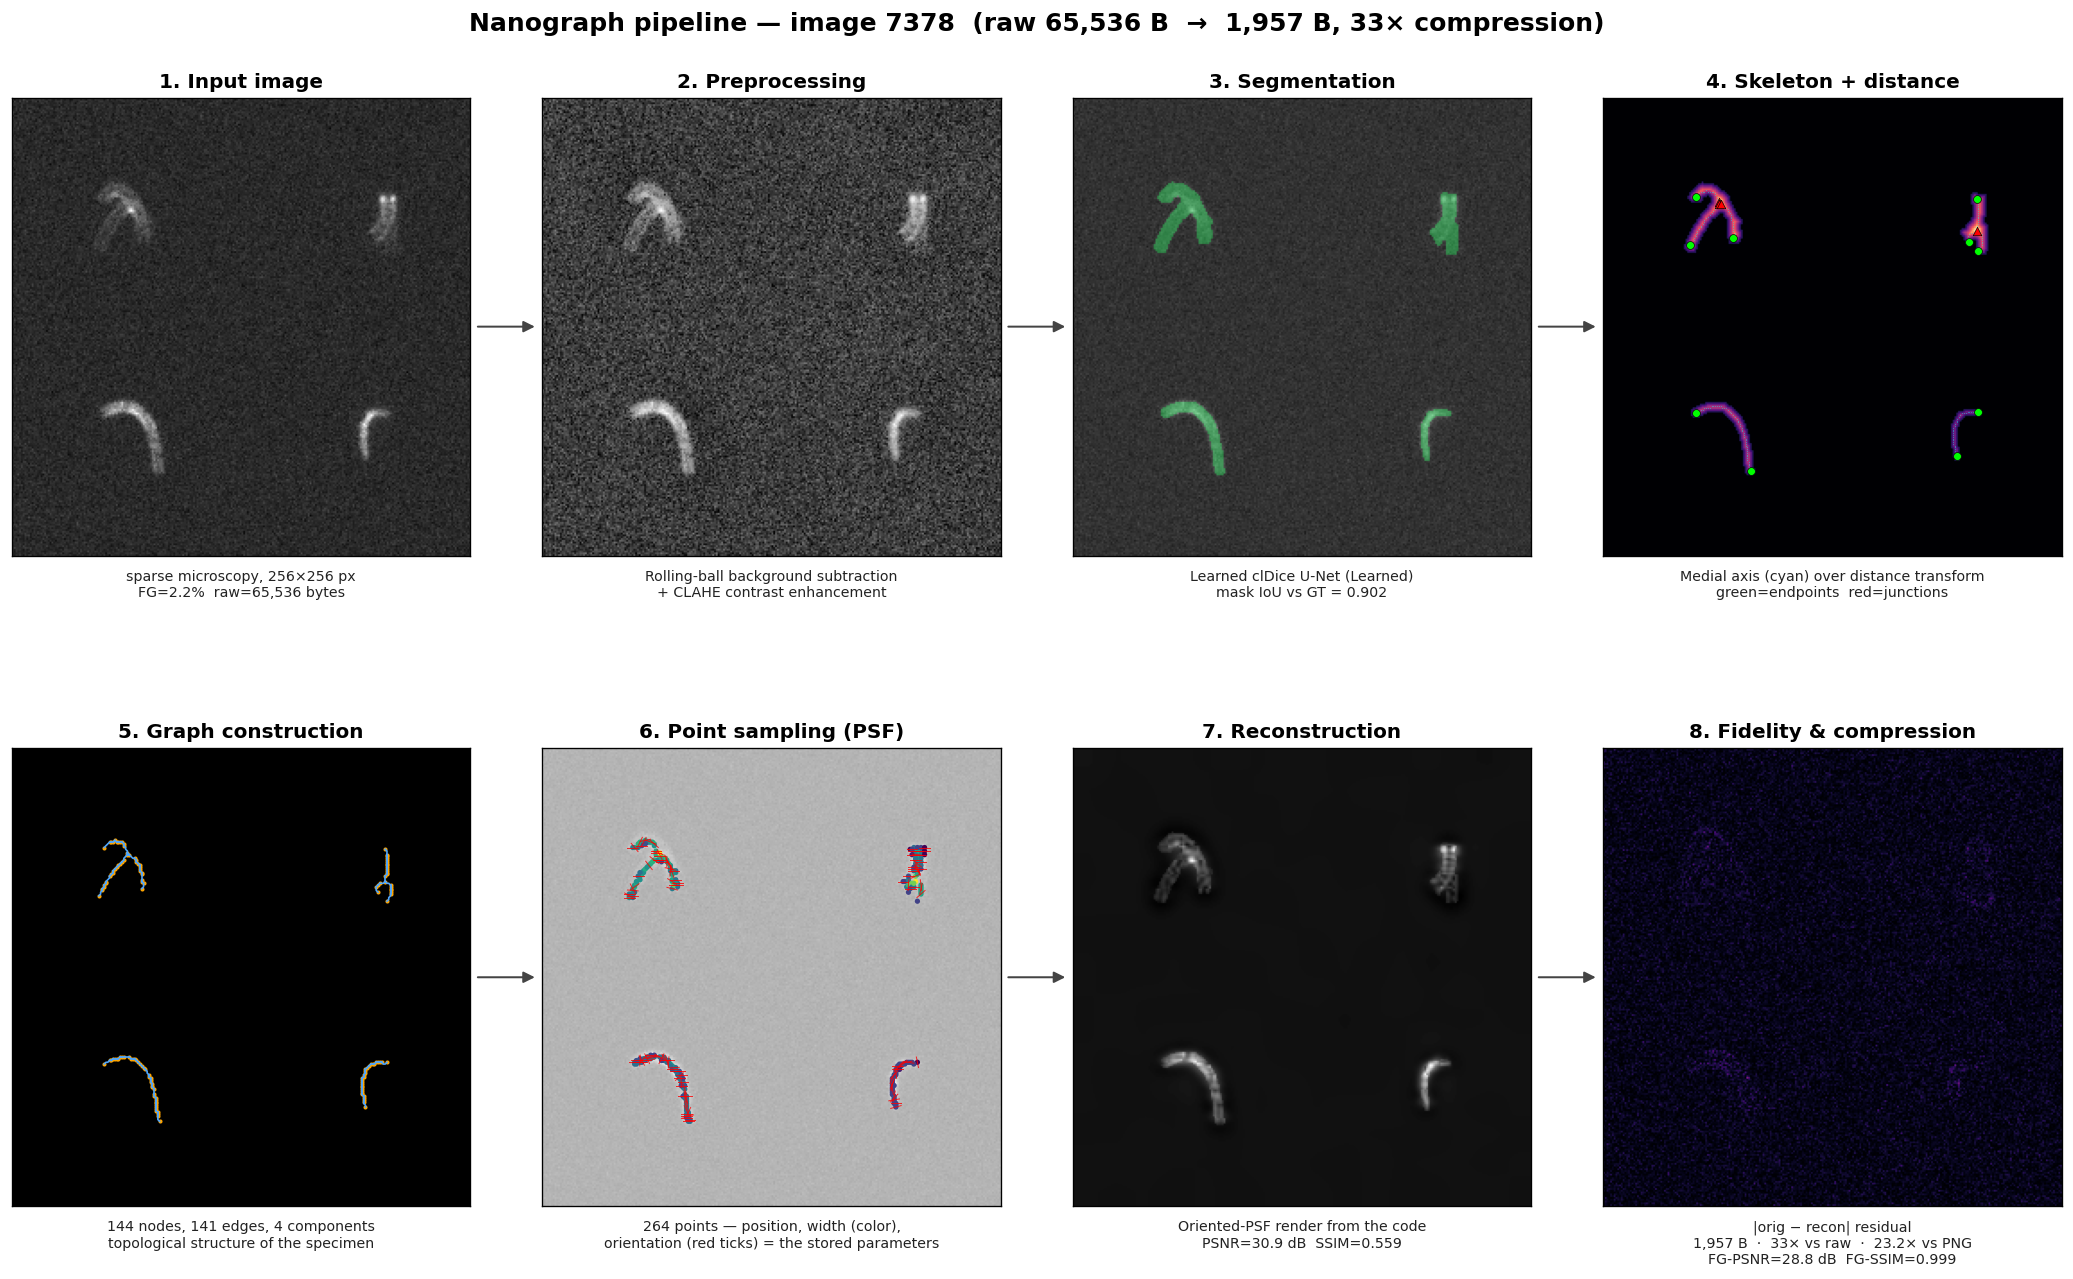
\includegraphics[width=\textwidth]{figures/pipeline_overview.png}
\caption{\method pipeline on a fluorescence organelle image: input,
preprocessing, foreground segmentation, skeleton with distance transform,
attributed graph, oriented-PSF point sampling, reconstruction and fidelity. The
image is stored as the graph (here 264 nodes, 1957\,bytes, $33\times$
compression, 30.9\,dB PSNR).}
\label{fig:overview}
\end{figure}

\subsection{Preprocessing and foreground segmentation}
The image is background-subtracted with a rolling-ball estimator~\cite{ballpark}
and locally contrast-normalised (CLAHE). Foreground is then extracted by a cascade of cheap
segmenters---Otsu thresholding and the Frangi~\cite{frangi} and
Meijering~\cite{meijering} vesselness filters---ranked by a
segmentation-quality score with early exit. Because thresholding tends to
over-predict (high recall, low precision), we add a learned candidate: a compact
U-Net~\cite{unet} trained with a combined Dice+BCE and clDice~\cite{cldice}
centreline loss. The centreline term specifically penalises breaks in thin
structure that area-weighted Dice ignores. The learned mask competes with the
classical cascade under a plausibility gate on foreground fraction, so it wins on
structure it was trained for and defers otherwise (Sec.~\ref{sec:seg}).

\subsection{Skeleton, graph, and sampling}
The foreground mask is skeletonised and its Euclidean distance transform gives a
per-pixel width. We trace branches between junctions and endpoints to build an
attributed graph $G=(V,E)$: each node $v\in V$ stores position, width,
intensity, and a tangent orientation estimated from a smoothed structure tensor;
each edge $e\in E$ stores its endpoints, pixel length, mean width, mean intensity
and curvature. Nodes are sub-sampled along branches at a spacing proportional to
local width, giving a variable-density point set that is denser where geometry
changes fastest.

\subsection{Oriented-PSF reconstruction}
Filaments are anisotropic, so isotropic Gaussians waste energy perpendicular to
the structure. \method reconstructs by convolving each sampled node with an
\emph{elliptical} PSF whose major axis is aligned to the node orientation
(default aspect ratio $2.5$) and whose scale follows the node width. Points are
grouped by (scale, orientation) bins for efficient FFT convolution. A
$16\times16$ bilinearly-upsampled background grid (256\,bytes) restores the
low-frequency field that a single mean value cannot, and an optional DCT residual
recovers fine foreground detail.

\subsection{Compression}
The graph is serialised as quantised node attributes---position (delta-coded
along branches), width, intensity, and a 1-byte orientation (256 levels over
$[0,\pi)$, quantisation error $<0.4^\circ$)---plus edge connectivity and the
background grid, then zlib-compressed. A typical organelle image costs
$\approx$\,7\,bytes/node.

% =====================================================================
\section{Representation fidelity and compression}\label{sec:repr}
% =====================================================================
\noindent\textbf{Data and metrics.} We evaluate on 726 fluorescence organelle
images with foreground annotations. We report full-image PSNR/SSIM,
foreground-restricted FG-PSNR/FG-SSIM, reconstruction IoU (thresholded recon vs.\
ground-truth foreground), payload size in bytes, and graph statistics. As a
compression baseline we encode each image with JPEG at the quality that matches
\method's byte budget, and compare fidelity at equal bytes.

\begin{table}[t]
\centering
\caption{\method on 726 organelle images (mean$\pm$std). Right: fraction of
images where \method beats \emph{byte-matched} JPEG.}
\label{tab:nmi}
\setlength{\tabcolsep}{5pt}
\begin{tabular}{lccc}
\toprule
Metric & \method & & vs.\ byte-matched JPEG \\
\midrule
Payload (bytes)      & $2469\pm331$   & Recon IoU wins   & $557/726$ (77\%)\\
Full PSNR (dB)       & $30.74\pm0.53$ & GT-IoU wins      & $354/726$ (49\%)\\
FG-PSNR (dB)         & $28.38\pm0.35$ & \multicolumn{2}{l}{}\\
FG-SSIM              & $0.997\pm0.001$& \multicolumn{2}{l}{}\\
Recon IoU            & $0.433\pm0.089$& \multicolumn{2}{l}{}\\
Nodes / image        & $336\pm52$     & \multicolumn{2}{l}{}\\
Encode time (ms)     & $625\pm43$     & \multicolumn{2}{l}{}\\
\bottomrule
\end{tabular}
\end{table}

\method encodes each image in $\approx$\,2.5\,kB and reconstructs foreground at
28.4\,dB FG-PSNR and 0.997 FG-SSIM (Table~\ref{tab:nmi}). At an \emph{equal byte
budget} it reconstructs the biological foreground more faithfully than JPEG on
77\% of images by reconstruction IoU, because it spends its bits on structure
rather than background texture. Unlike a codec, the same payload directly yields
morphometry (mean width $4.3\pm0.5$\,px, total edge length, junction-degree
statistics) and topology ($\beta_0$ components, $\beta_1$ cycles) without any
re-processing.

% =====================================================================
\section{Cross-modality generality}\label{sec:cross}
% =====================================================================
We apply the \emph{same} encoder, unchanged, to four further modalities:
Cells3D membrane and nuclei, retinal vessels, and fluorescence cells
(Table~\ref{tab:cross}). Foreground fidelity remains high (FG-SSIM
$0.97$--$0.99$, FG-PSNR $27$--$34$\,dB) and \method beats byte-matched JPEG on
reconstruction IoU for 82--100\% of images across datasets, confirming that the
graph representation is not specific to organelles.

\begin{table}[t]
\centering
\caption{Same encoder across five modalities. FG fidelity and IoU-wins vs.\
byte-matched JPEG.}
\label{tab:cross}
\setlength{\tabcolsep}{4pt}
\begin{tabular}{lccccc}
\toprule
 & Organelles & Cells3D mem. & Cells3D nuc. & Retina & Cells \\
$N$ & 726 & 60 & 60 & 25 & 5\\
\midrule
FG-SSIM       & 0.997 & 0.982 & 0.967 & 0.985 & 0.984\\
FG-PSNR (dB)  & 28.4  & 31.2  & 27.2  & 33.1  & 34.5\\
IoU wins/JPEG & 77\%  & 82\%  & 83\%  & 88\%  & 100\%\\
\bottomrule
\end{tabular}
\end{table}

% =====================================================================
\section{The segmentation bottleneck and cross-domain generalisation}\label{sec:seg}
% =====================================================================
Reconstruction fidelity is upper-bounded by the foreground mask. The classical
cascade over-predicts: on the organelle set it reaches segmentation IoU $0.489$
with recall $0.983$ but precision only $0.493$. Replacing it by the clDice U-Net
(candidate mode, light cleaning that preserves thin structure) raises
\emph{leakage-free held-out} segmentation IoU from $0.381$ (classical) to
$0.875$, with precision and recall both $\approx0.93$ (Table~\ref{tab:seg}).

\begin{table}[t]
\centering
\caption{Held-out segmentation on organelles (seed-fixed val split).}
\label{tab:seg}
\setlength{\tabcolsep}{7pt}
\begin{tabular}{lcccc}
\toprule
Front end & IoU & Precision & Recall & F1\\
\midrule
Classical cascade      & 0.381 & 0.440 & 0.850 & 0.540\\
clDice U-Net (learned) & \textbf{0.875} & 0.933 & 0.931 & 0.929\\
\bottomrule
\end{tabular}
\end{table}

\noindent\textbf{Out-of-domain failure.} A network trained only on
bright-on-dark organelles transfers poorly to other curvilinear modalities. On
four external datasets---STARE and DRIVE retinal vessels~\cite{stare,drive},
EPFL/Lucchi electron-microscopy mitochondria~\cite{lucchi}, and IRM
microtubules---the whole pipeline collapses (Table~\ref{tab:retrain}, ``old'').
We trace this to three compounding causes: (i)~\emph{polarity}---external
structures are dark-on-bright, the opposite of fluorescent organelles, so
vesselness filters and the organelle network respond to background; (ii)~the
organelle-calibrated quality score cannot \emph{rank} candidate masks on these
modalities; and (iii)~EM mitochondria are filled objects in dense neuropil, not
separable by any threshold or ridge filter (an oracle dark-ridge Frangi reaches
only 0.076 IoU).

\noindent\textbf{Polarity-agnostic multi-domain retraining.} We retrain a single
clDice U-Net on all four datasets jointly, with a \emph{random-inversion}
augmentation that shows every structure in both polarities, so the network
segments a structure whether it appears bright or dark and needs no
inference-time polarity detector. Splits are leakage-free (independent images
for vessels/filaments; a contiguous held-out slice block with a guard gap for
the EM volume). This restores segmentation across all four domains
(Table~\ref{tab:retrain}): held-out IoU rises to 0.64/0.56/0.60 on
vessels/filaments and to \textbf{0.82} on EM mitochondria---from $0.001$. We
verify the network is genuinely polarity-agnostic: feeding images as-is matches
an oracle that picks the better of both polarities per image (e.g.\ 0.643 vs.\
0.643 on STARE). The retrained weight drops into the pipeline as a
\texttt{for\_curvilinear} preset and reproduces these numbers end-to-end.

\begin{table}[t]
\centering
\caption{Held-out segmentation IoU on four out-of-domain curvilinear datasets:
classical/in-domain pipeline (``old'') vs.\ the polarity-agnostic multi-domain
retraining (``ours'').}
\label{tab:retrain}
\setlength{\tabcolsep}{7pt}
\begin{tabular}{lcccc}
\toprule
 & STARE & DRIVE & Microtubules & EPFL mito (EM)\\
\midrule
Old (classical / in-domain) & 0.056 & 0.100 & 0.021 & 0.001\\
Ours (retrained)            & \textbf{0.643} & \textbf{0.564} & \textbf{0.599} & \textbf{0.822}\\
\bottomrule
\end{tabular}
\end{table}

\begin{figure}[t]
\centering
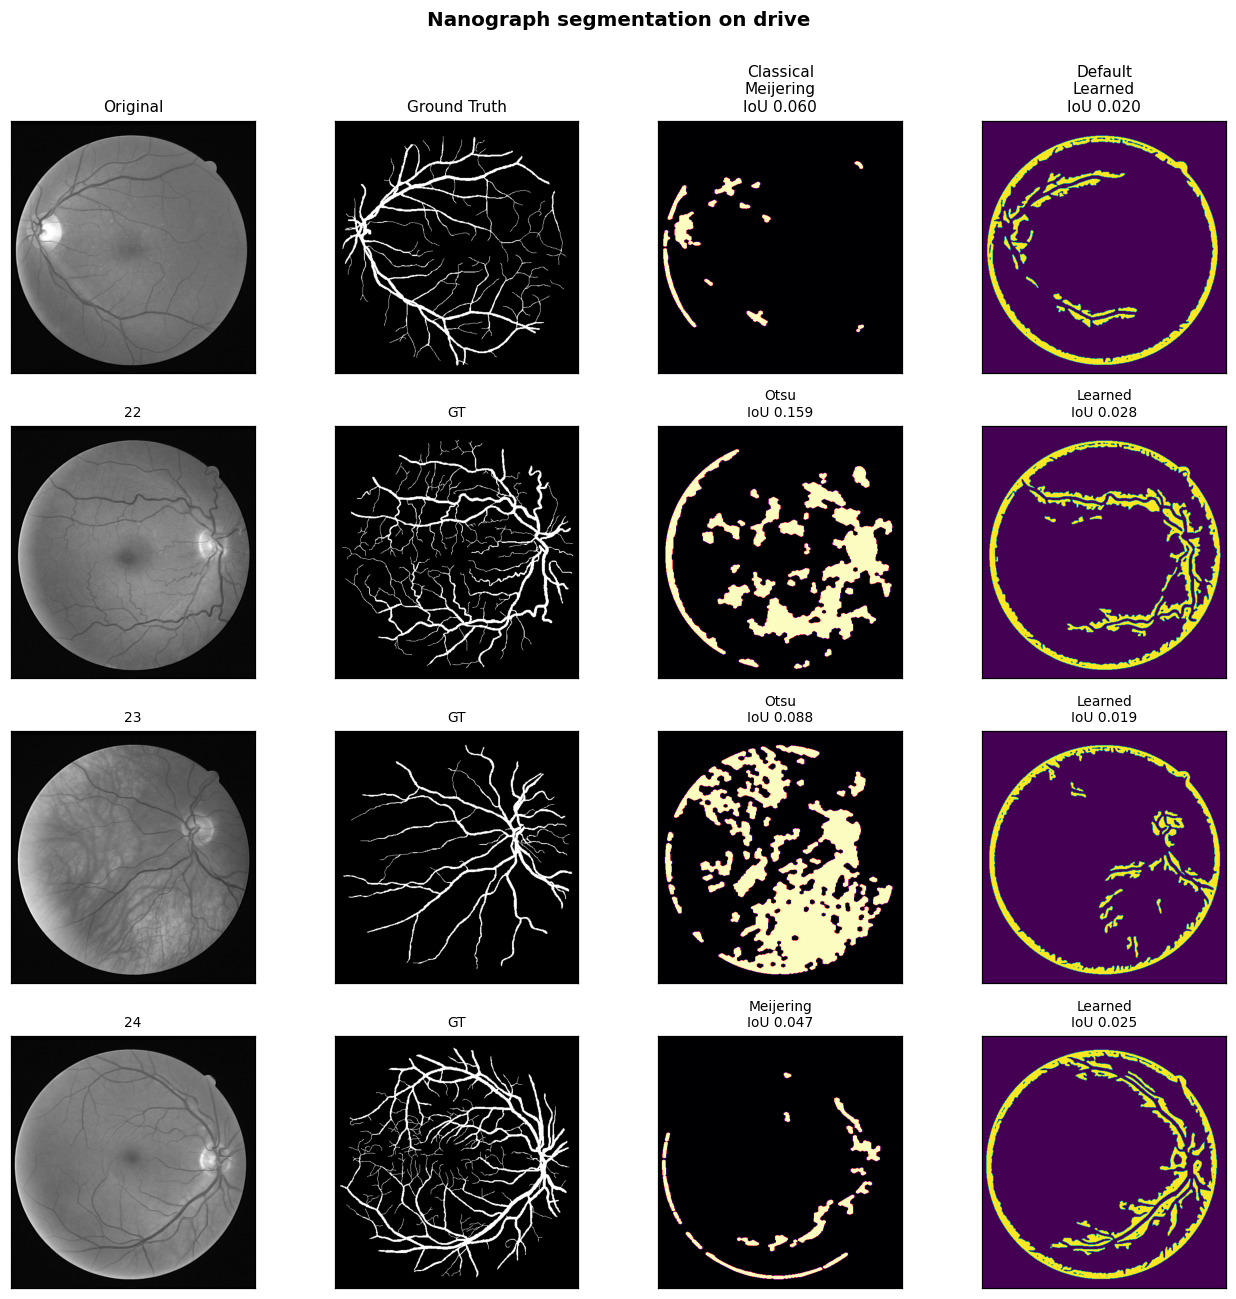
\includegraphics[width=0.86\textwidth]{figures/ext_drive.png}
\caption{Held-out DRIVE retinal vessels: input, ground truth, and the retrained
\method segmentation used by the encoder.}
\label{fig:drive}
\end{figure}

% =====================================================================
\section{Discussion and limitations}
% =====================================================================
\method treats a curvilinear image as an attributed graph, which unifies
compression, morphometry and topology under one object and makes the geometry a
first-class, queryable artefact. The representation is lossy by design: full-image
SSIM is modest because texture and non-curvilinear content are not modelled, and
reconstruction IoU is bounded by segmentation. The external datasets are small
(16 training images for STARE/DRIVE), so their numbers, though leakage-free, are
single-split estimates; the EM result is on correlated slices from one volume
with a guard-gap split. The polarity-agnostic retraining is an input-representation
fix, not a claim of universal segmentation. Natural extensions are 3-D graphs,
temporal graph tracking (already scaffolded), and graph-native downstream models.

% =====================================================================
\section{Conclusion}
% =====================================================================
We presented \method, a structural graph representation for curvilinear
microscopy that is compact, analysable and reconstructable in one object. It
compresses competitively with JPEG at equal bytes while exposing morphometry and
topology for free, transfers across modalities, and---with a polarity-agnostic
multi-domain segmenter---restores fidelity on out-of-domain vessels, filaments
and electron-microscopy mitochondria.

% ---------------------------------------------------------------------
\bibliographystyle{splncs04}
\bibliography{references}

\end{document}
